\documentclass[12pt, oneside]{article}   	% use "amsart" instead of "article" for
\usepackage[left=2.7cm,right=2.7cm,top=2.7cm,bottom=2.7cm]{geometry}	

\usepackage{graphicx}		
\usepackage{amssymb}
\usepackage{amsmath}
\usepackage[font=normalsize]{caption}
\usepackage{subcaption}
\usepackage{float}

\setlength{\parindent}{0pt}
\begin{document}
1)\par
\begin{flalign*}
&P(X^1_S = 1|X^1_{\partial S}) = \frac{e^{\beta \sum_{<1,t>} 1(1 = X_t^1)}}{e^{\beta \sum_{<1,t>} 1(1 = X_t^1)} + e^{\beta \sum_{<1,t>} 1(0 = X_t^1)}} &\\
&P(X^2_S = 1|X^2_{\partial S}) = \frac{e^{\beta \sum_{<1,t>} 1(1 = X_t^2)}}{e^{\beta \sum_{<1,t>} 1(1 = X_t^2)} + e^{\beta \sum_{<1,t>} 1(0 = X_t^2)}} &
\end{flalign*}
We generate a uniform random variable $r$ from $[0, 1]$.  If $0<r \leq P(X^1_S = 1|X^1_{\partial S})$, $X^1_S=1$ and if $P(X^1_S = 1|X^1_{\partial S}) < r \leq 1$, $X^1_S=0$.  If $0<r \leq P(X^2_S = 1|X^2_{\partial S})$, $X^2_S=1$ and if $P(X^2_S = 1|X^2_{\partial S}) < r \leq 1$, $X^2_S=0$.Now we prove Q1 by induction. Initially we know $X_S^1 \geq X_S^2$ for every site. \par
Assume after $n$ states, it's still true that $X_S^1 \geq X_S^2$. For state $n+1$, we need to prove there is no case that $X_S^1 = 0$ and $X_S^2=1$. If $X_S^1 = 0$ and $X_S^2=1$, $r > P(X^1_S = 1|X^1_{\partial S}) = \frac{e^{\beta \sum_{<1,t>} 1(1 = X_t^1)}}{e^{\beta \sum_{<1,t>} 1(1 = X_t^1)} + e^{\beta \sum_{<1,t>} 1(0 = X_t^1)}}$ and  $r \leq P(X^2_S = 1|X^2_{\partial S}) = \frac{e^{\beta \sum_{<1,t>} 1(1 = X_t^2)}}{e^{\beta \sum_{<1,t>} 1(1 = X_t^2)} + e^{\beta \sum_{<1,t>} 1(0 = X_t^2)}}$. So if we can prove $P(X^1_S = 1|X^1_{\partial S}) \geq  P(X^2_S = 1|X^2_{\partial S})$, $X_S^1 = 0$ and $X_S^2=1$ cannot happen simultaneously.
\begin{flalign*}
&\frac{e^{\beta \sum_{<1,t>} 1(1 = X_t^1)}}{e^{\beta \sum_{<1,t>} 1(1 = X_t^1)} + e^{\beta \sum_{<1,t>} 1(0 = X_t^1)}} >  \frac{e^{\beta \sum_{<1,t>} 1(1 = X_t^2)}}{e^{\beta \sum_{<1,t>} 1(1 = X_t^2)} + e^{\beta \sum_{<1,t>} 1(0 = X_t^2)}} \Rightarrow &\\
&e^{\beta\sum 1(1=X_t^1) + \beta\sum 1(1=X_t^2)} +e^{\beta\sum 1(1=X_t^1) + \beta\sum 1(0=X_t^2)} \geq &\\
&\hspace{6cm} e^{\beta\sum 1(1=X_t^1) + \beta\sum 1(1=X_t^2)} + e^{\beta\sum 1(0=X_t^1) + \beta\sum 1(1=X_t^2)} \Rightarrow &\\
&\sum 1(1=X_t^1) + \sum 1(0=X_t^2) \geq \sum 1(0=X_t^1) + \sum 1(1=X_t^2) \quad (*)&
\end{flalign*}

\begin{flalign*}
& (*) =
\begin{cases}
X_t^1 = 1, X_t^2 = 1 \qquad 1(1=X_t^1) + 1(0=X_t^2) = 1 \geq 1 = 1(0=X_t^1) + 1(1=X_t^2)\\
X_t^1 = 1, X_t^2 = 0 \qquad 1(1=X_t^1) + 1(0=X_t^2) = 2 \geq 0 = 1(0=X_t^1) + 1(1=X_t^2)\\
X_t^1 = 0, X_t^2 = 0 \qquad 1(1=X_t^1) + 1(0=X_t^2) = 1 \geq 1 = 1(0=X_t^1) + 1(1=X_t^2)\\
X_t^1 = 0, X_t^2 = 1 \qquad\text{This case won't happen based on n-state induction}
\end{cases} &
\end{flalign*}
Now, the proof is finished. \par
2)\par
I attach R code and C++ code on CCLE. 
\begin{figure}[H]
        \centering
        \begin{subfigure}[b]{0.475\textwidth}
            \centering
            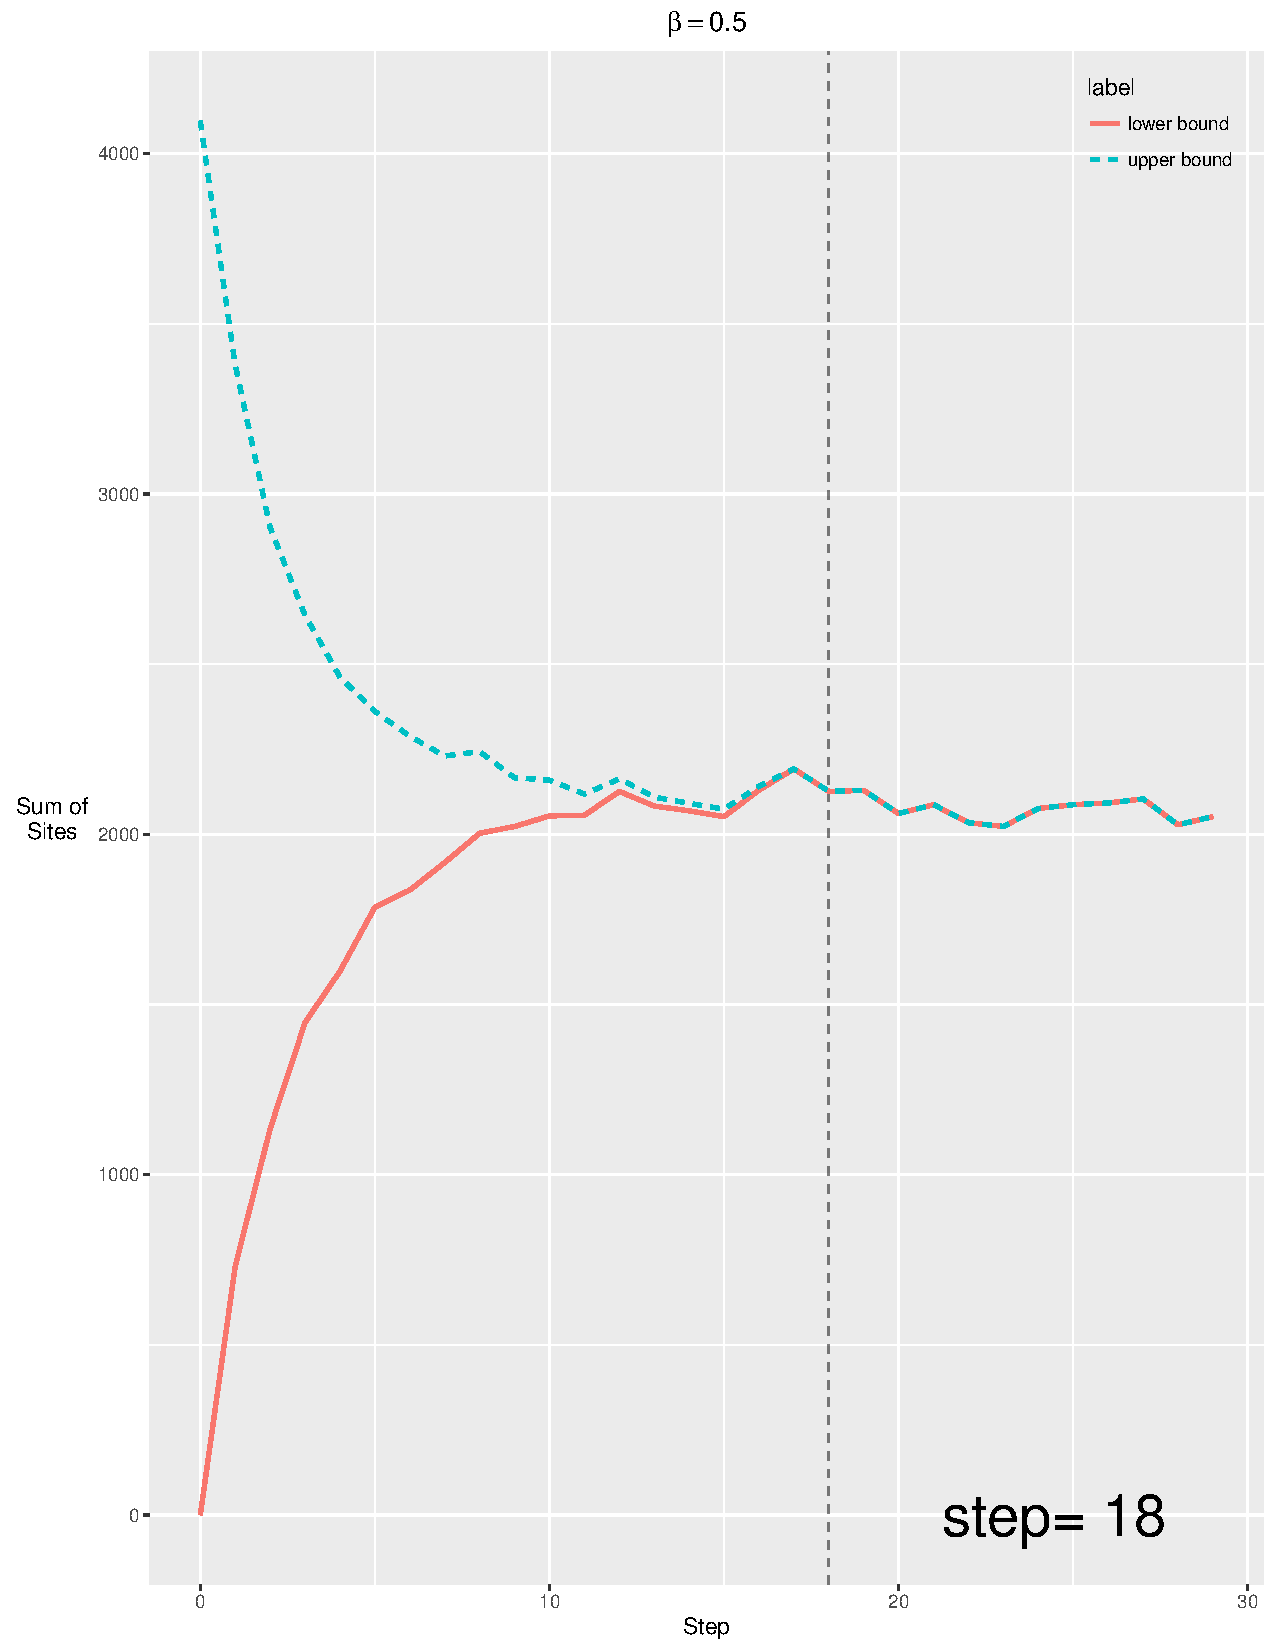
\includegraphics[width=\textwidth, height=0.5\textheight]{050.pdf}
        \end{subfigure}
        \quad
        \begin{subfigure}[b]{0.475\textwidth}
            \centering
            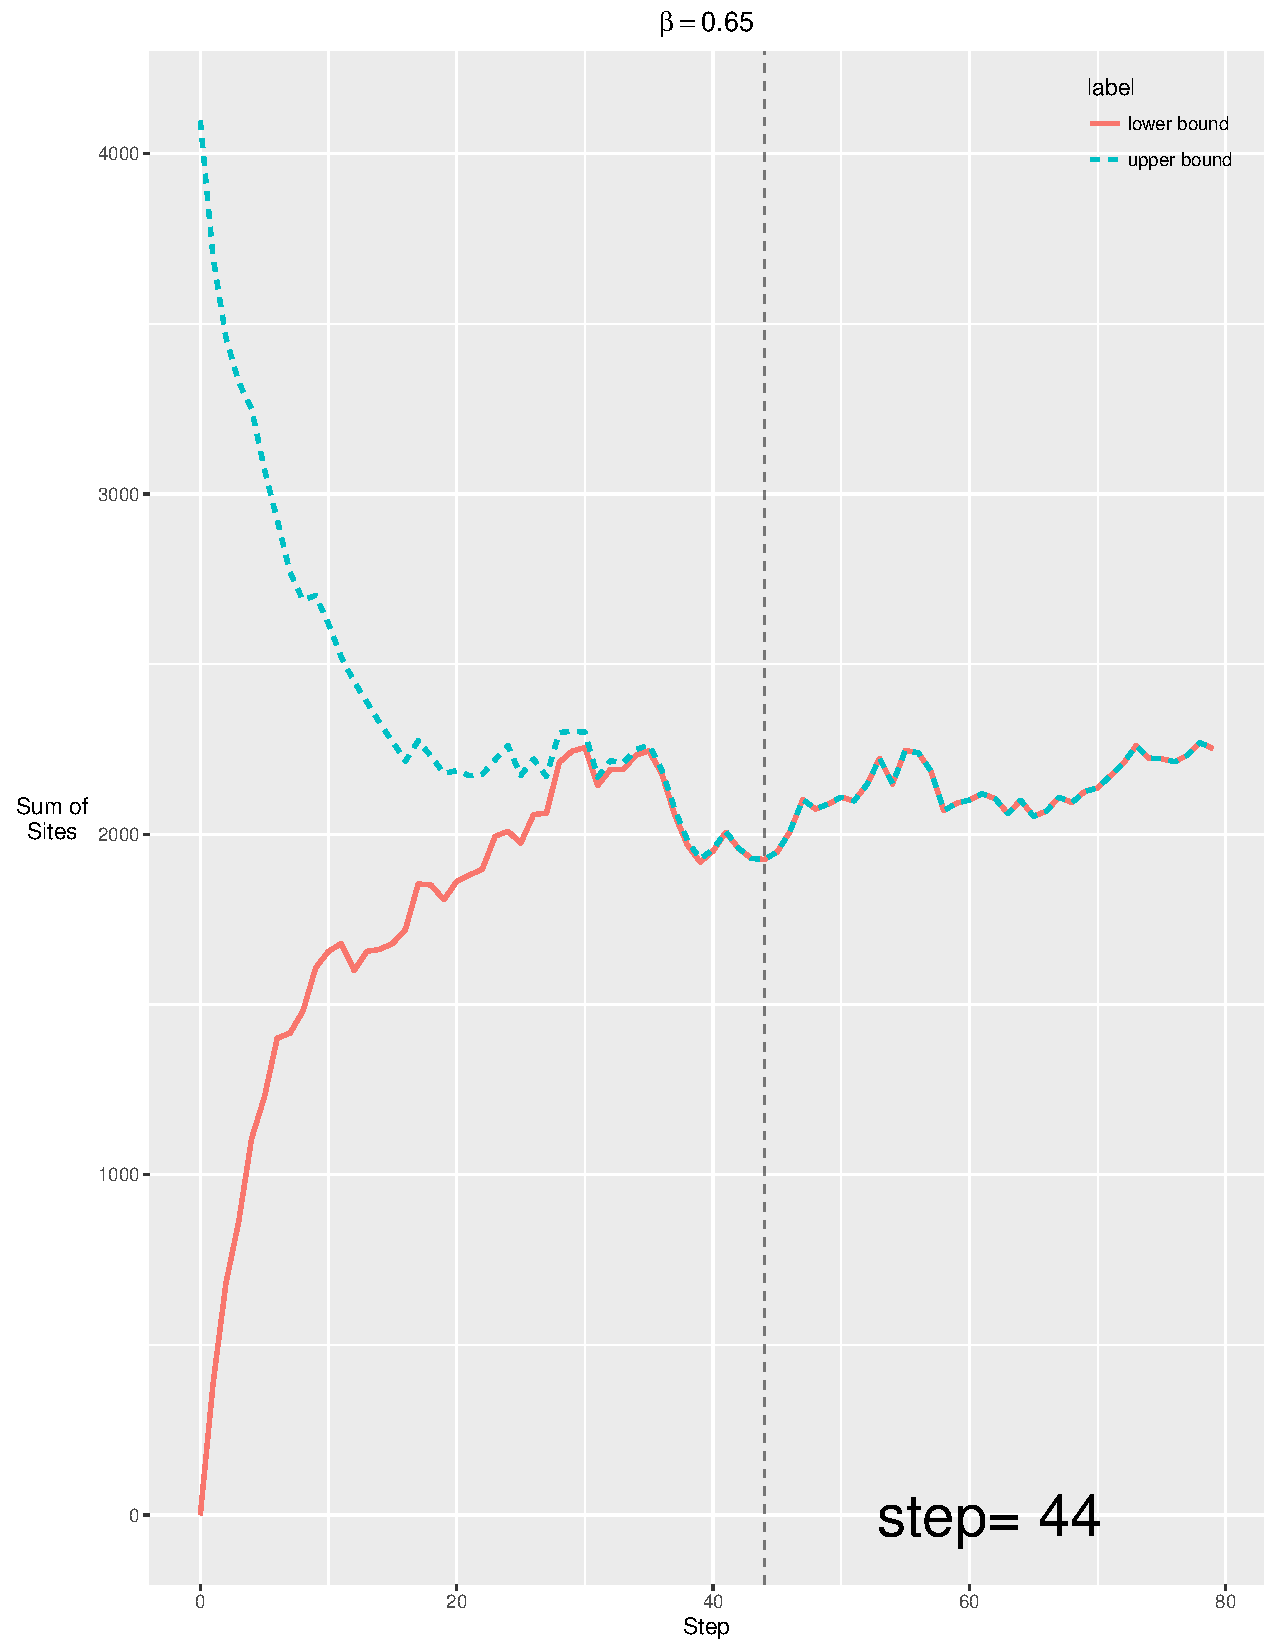
\includegraphics[width=\textwidth, height=0.5\textheight]{065.pdf}
        \end{subfigure} \\
        \centering
        \begin{subfigure}[b]{0.475\textwidth}
            \centering
            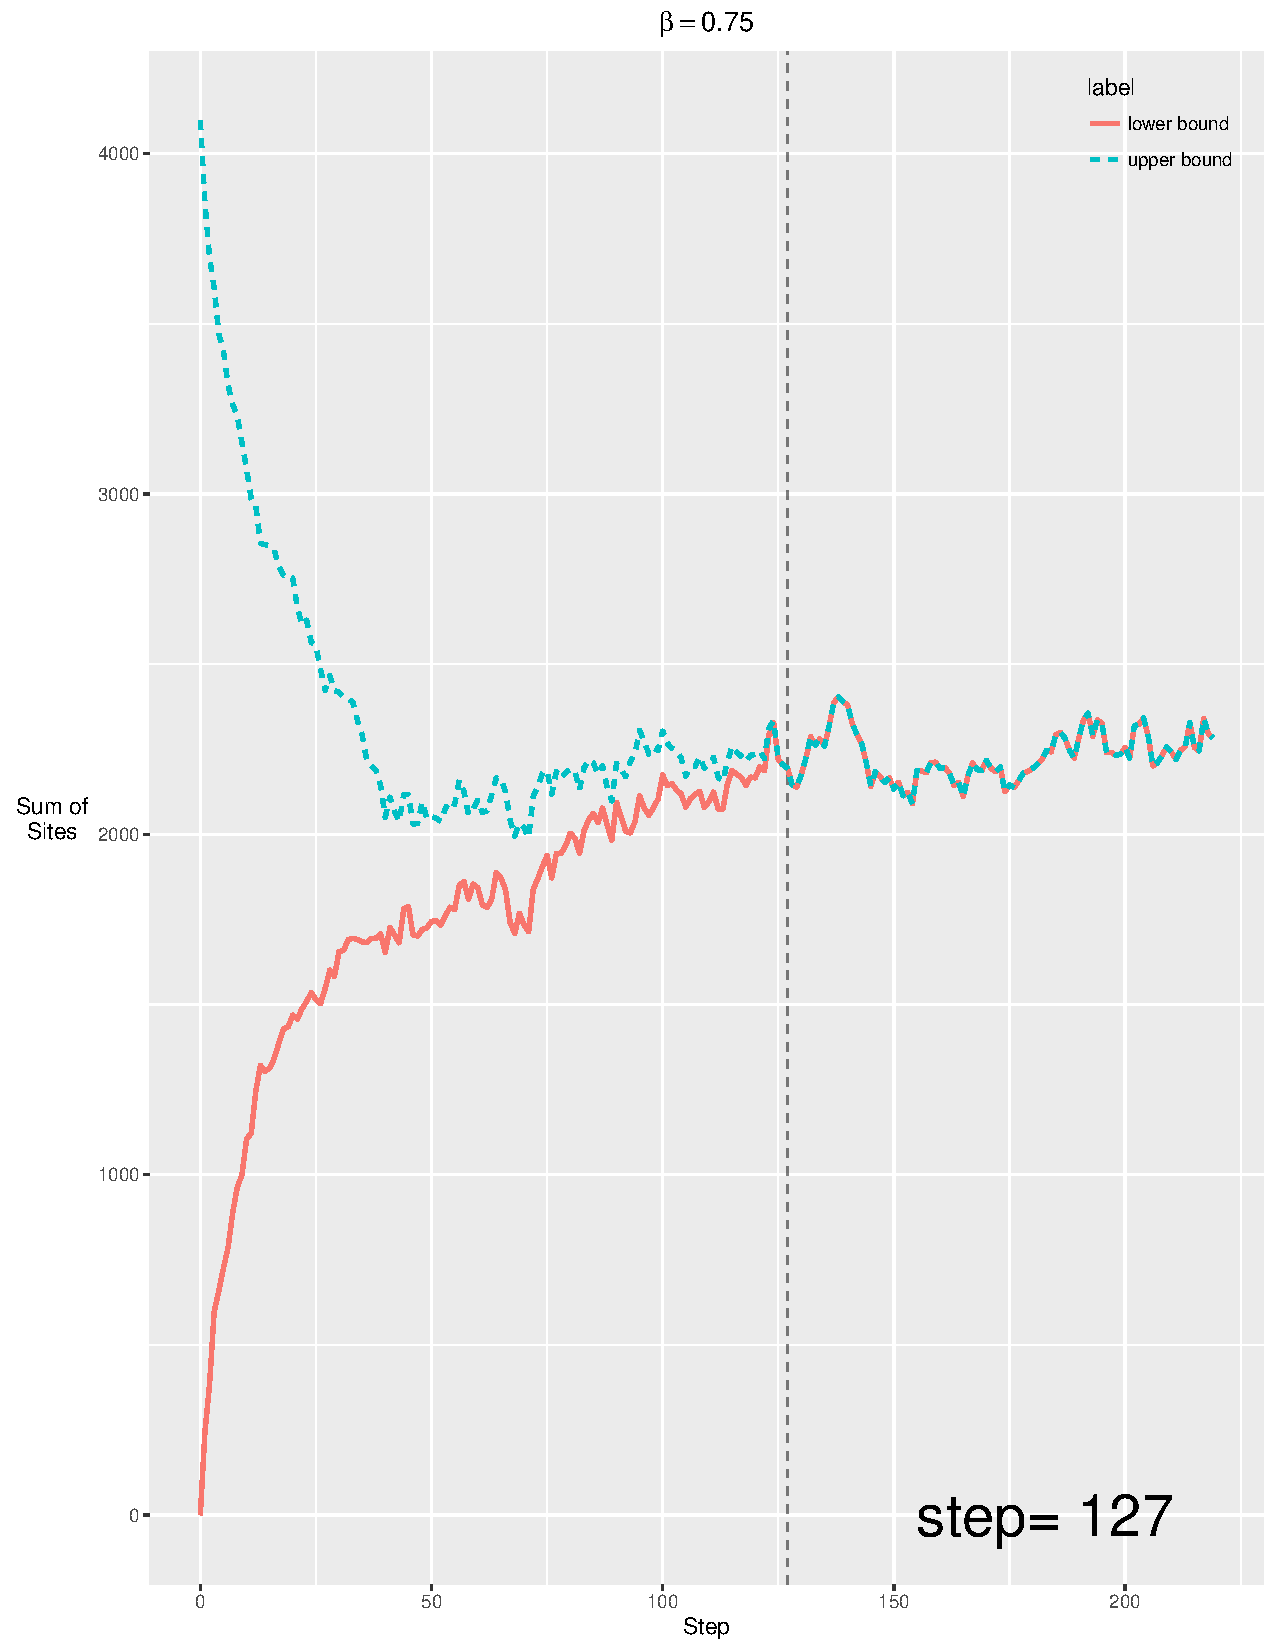
\includegraphics[width=\textwidth, height=0.5\textheight]{075.pdf}
        \end{subfigure}
        \quad
        \begin{subfigure}[b]{0.475\textwidth}
            \centering
            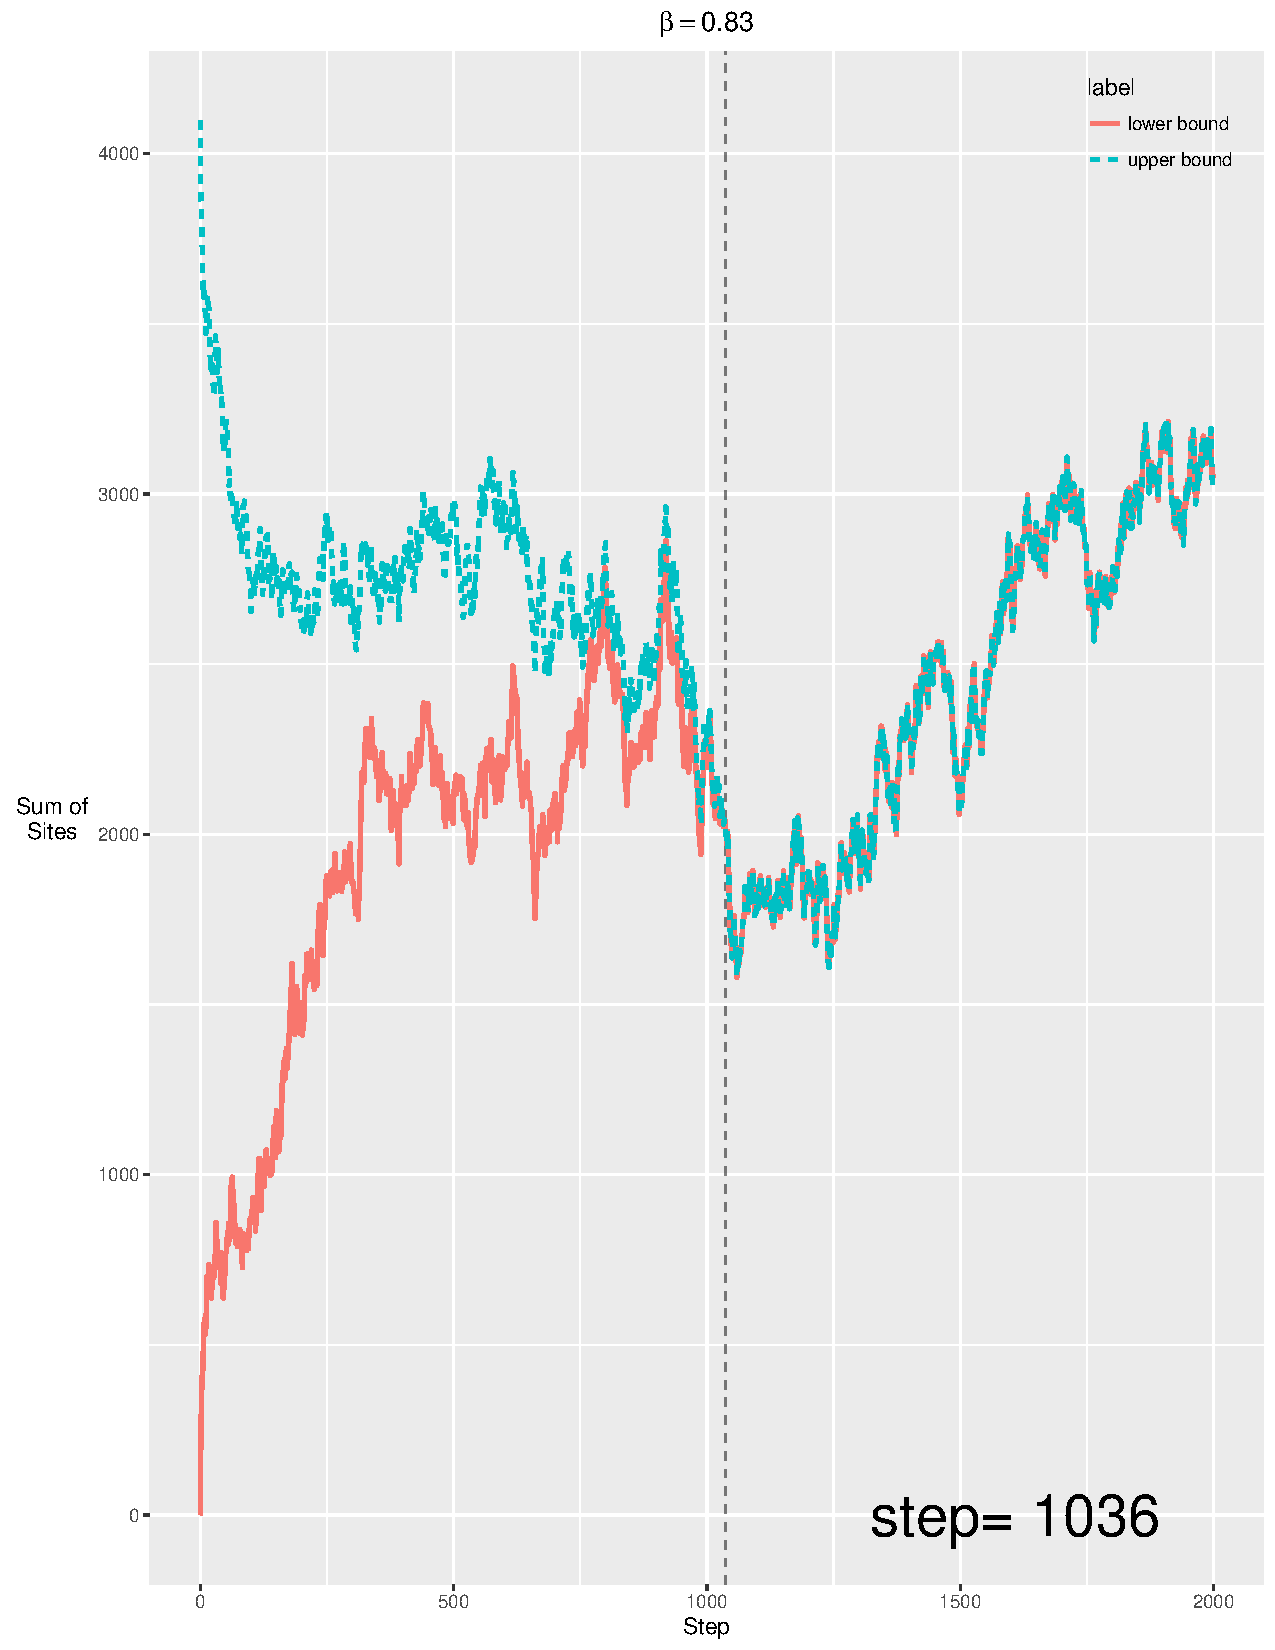
\includegraphics[width=\textwidth, height=0.5\textheight]{083.pdf}
        \end{subfigure} \\
\end{figure}
\begin{figure}[H]
        \centering
        \begin{subfigure}[b]{0.475\textwidth}
            \centering
            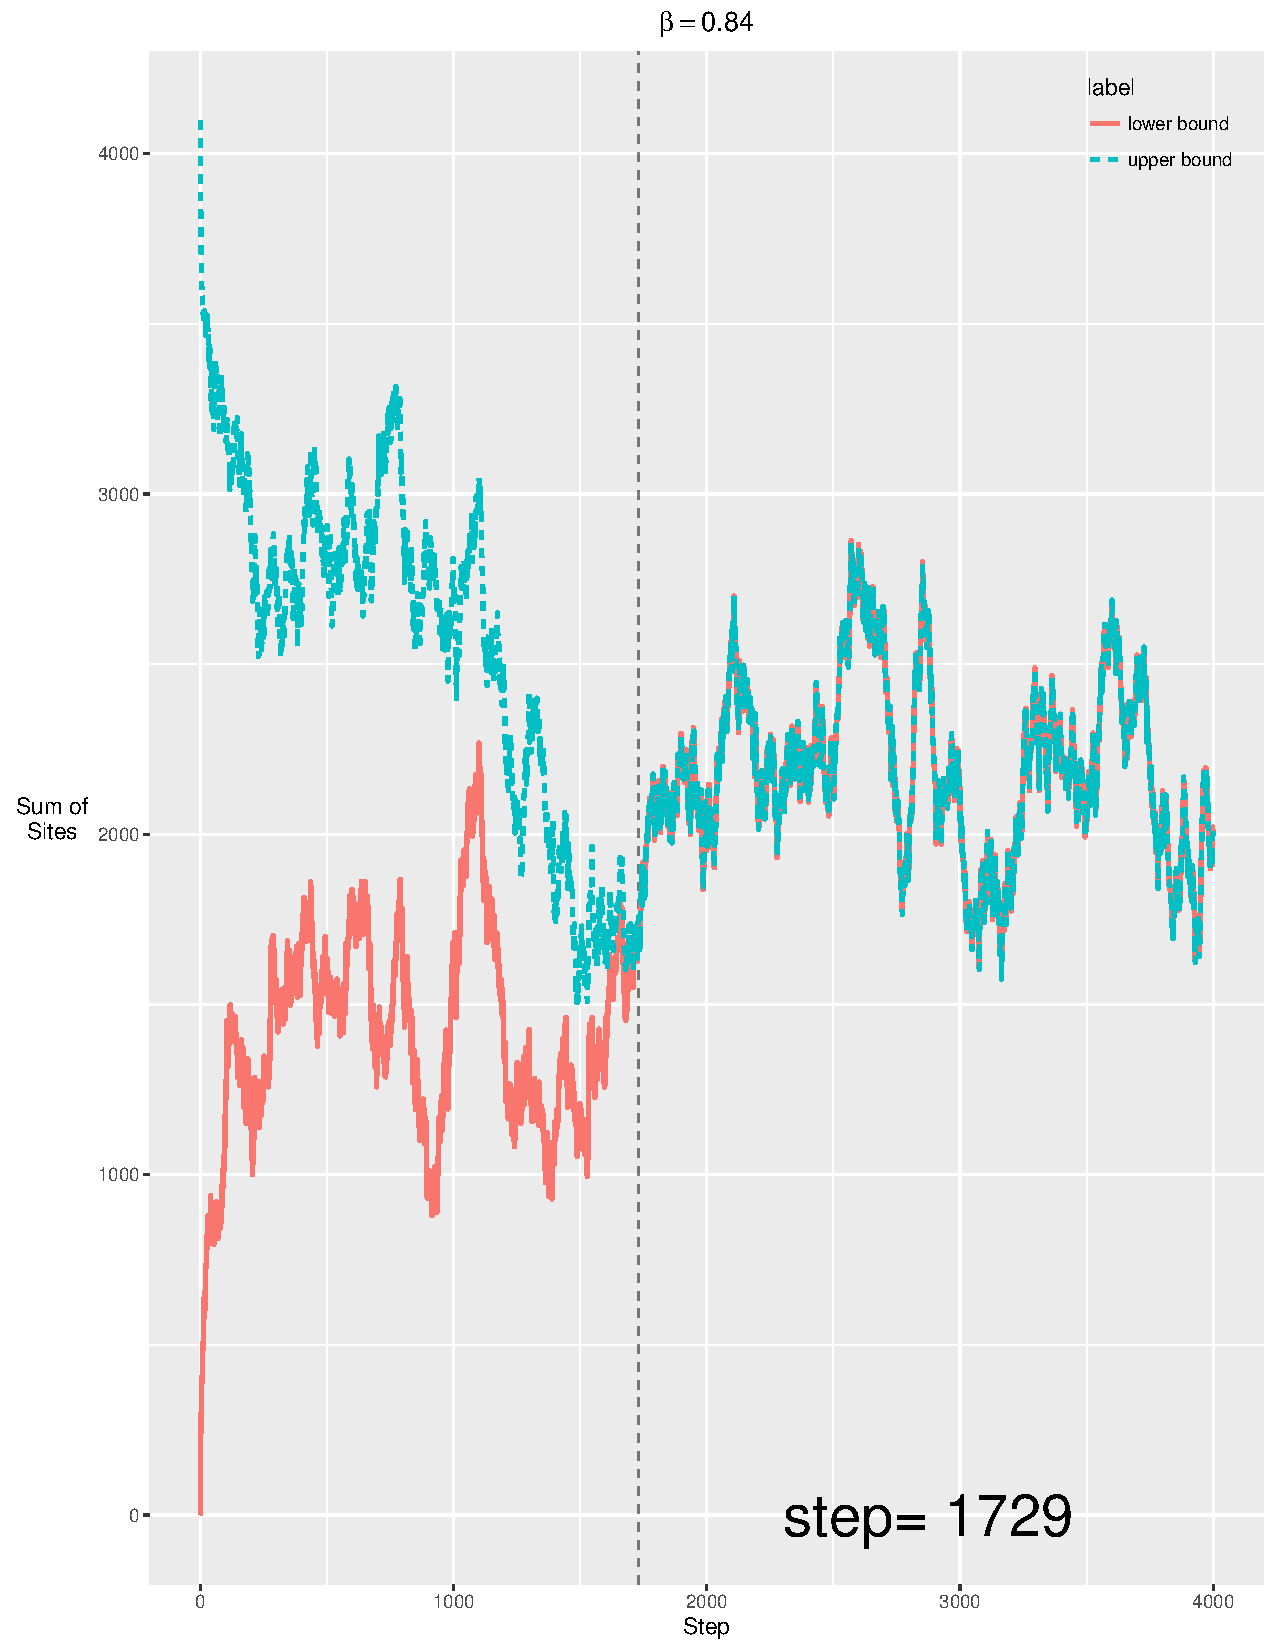
\includegraphics[width=\textwidth, height=0.5\textheight]{084.pdf}
        \end{subfigure}
        \quad
        \begin{subfigure}[b]{0.475\textwidth}
            \centering
            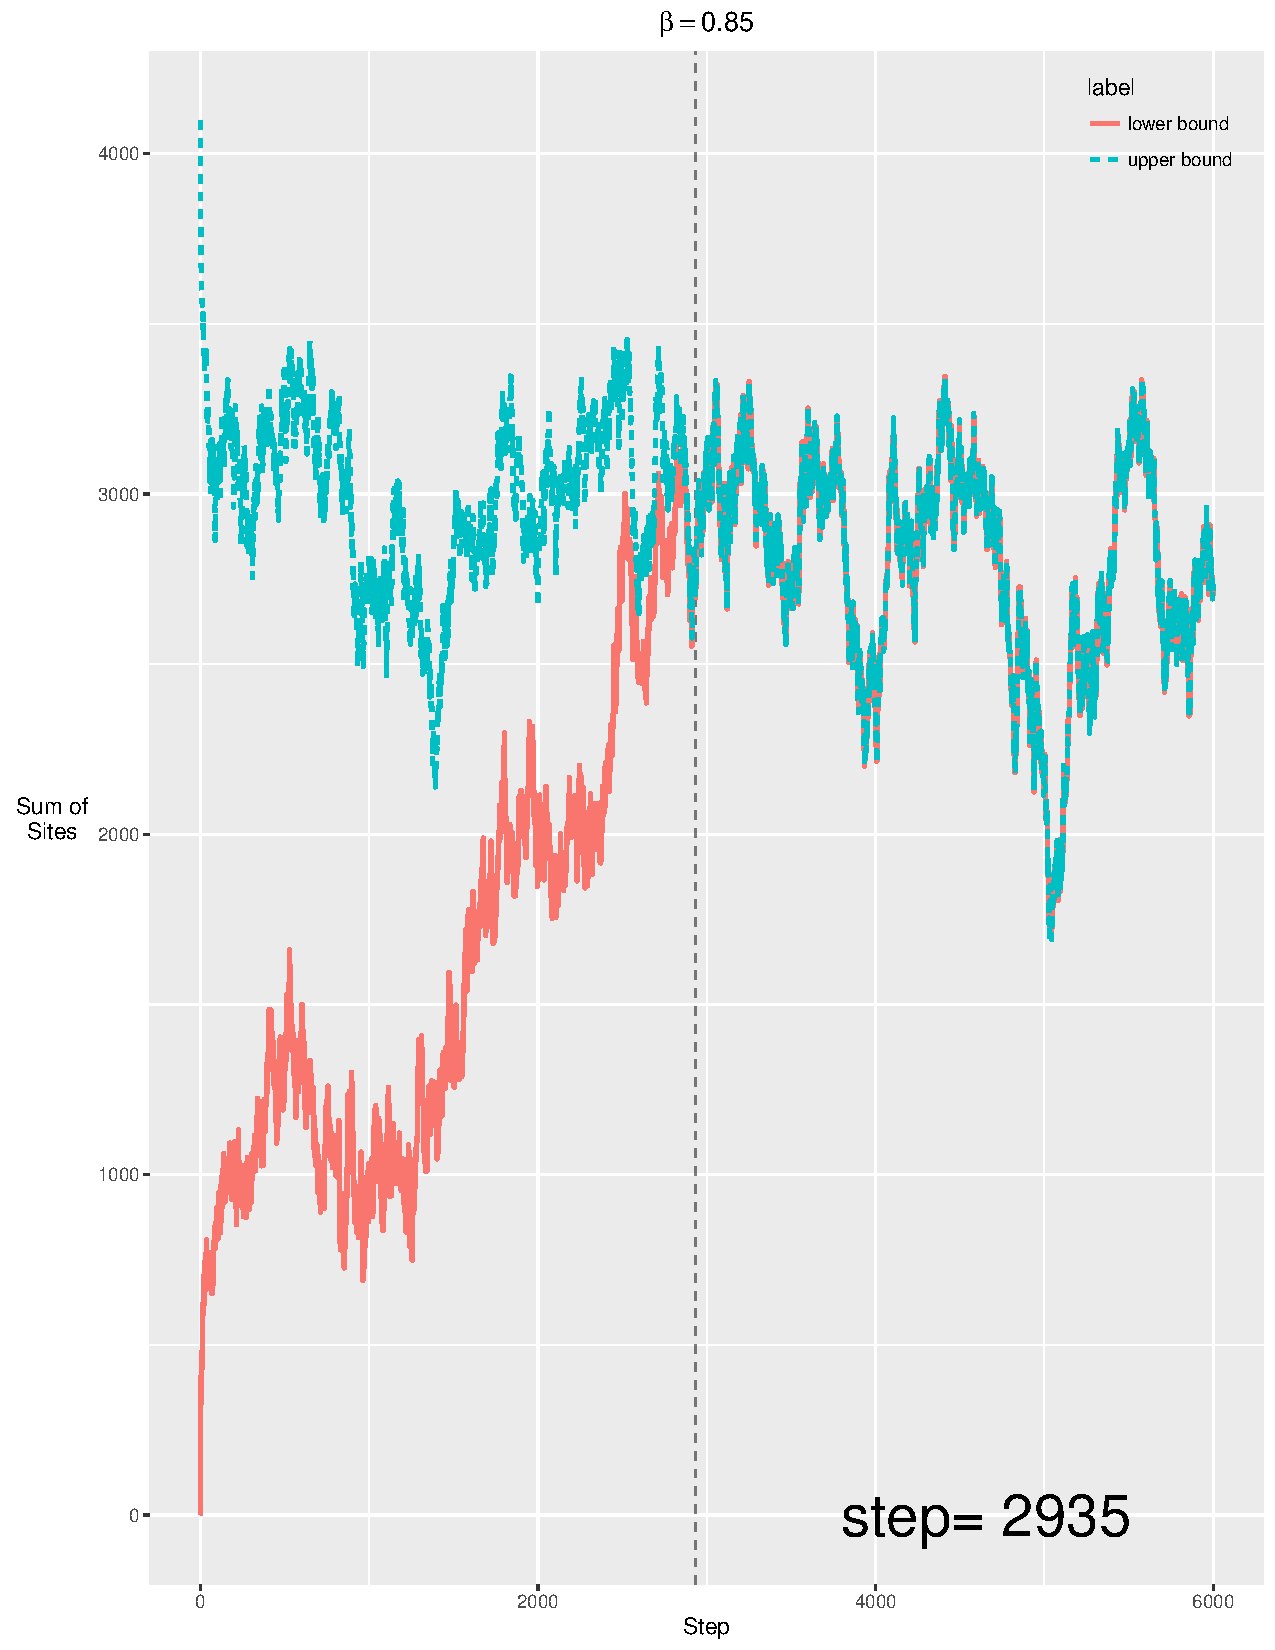
\includegraphics[width=\textwidth, height=0.5\textheight]{085.pdf}
        \end{subfigure} \\
        \centering
        \begin{subfigure}[b]{0.475\textwidth}
            \centering
            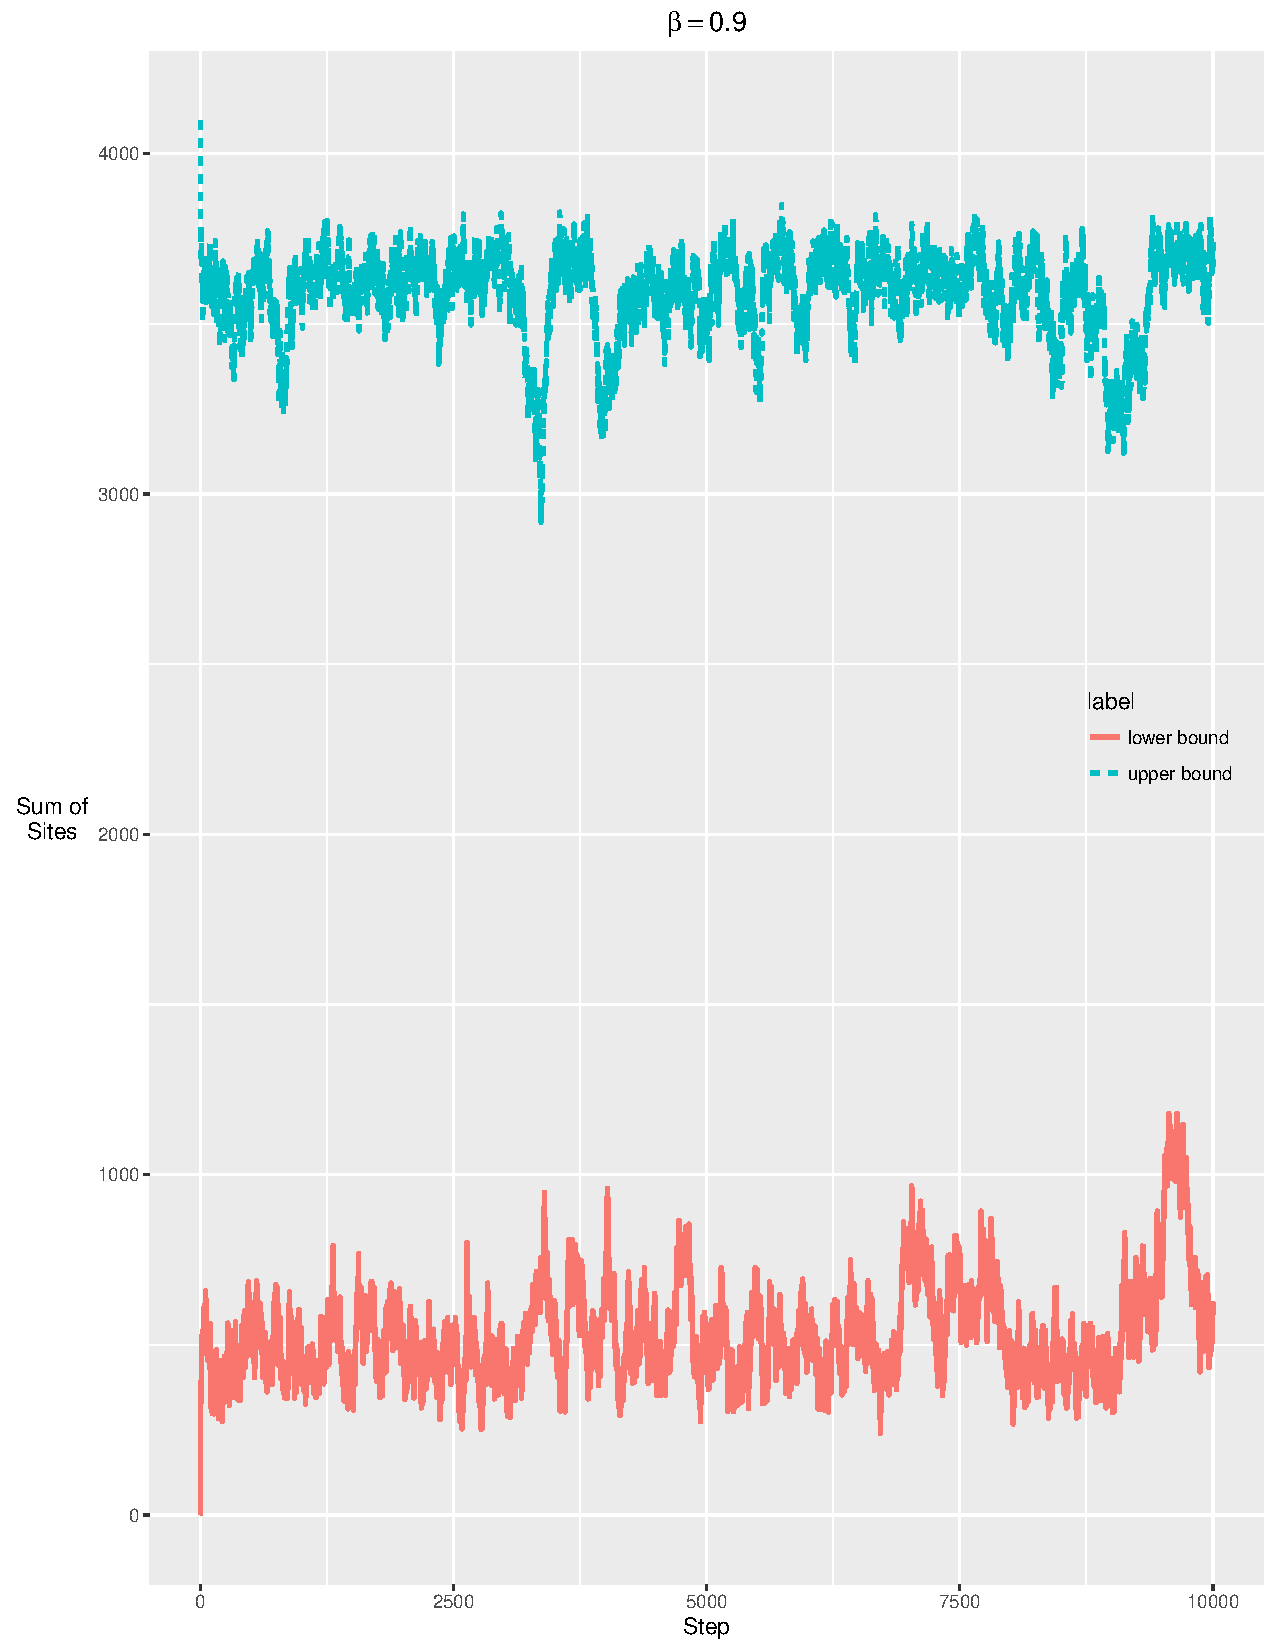
\includegraphics[width=\textwidth, height=0.5\textheight]{090.pdf}
        \end{subfigure}
        \quad
        \begin{subfigure}[b]{0.475\textwidth}
            \centering
            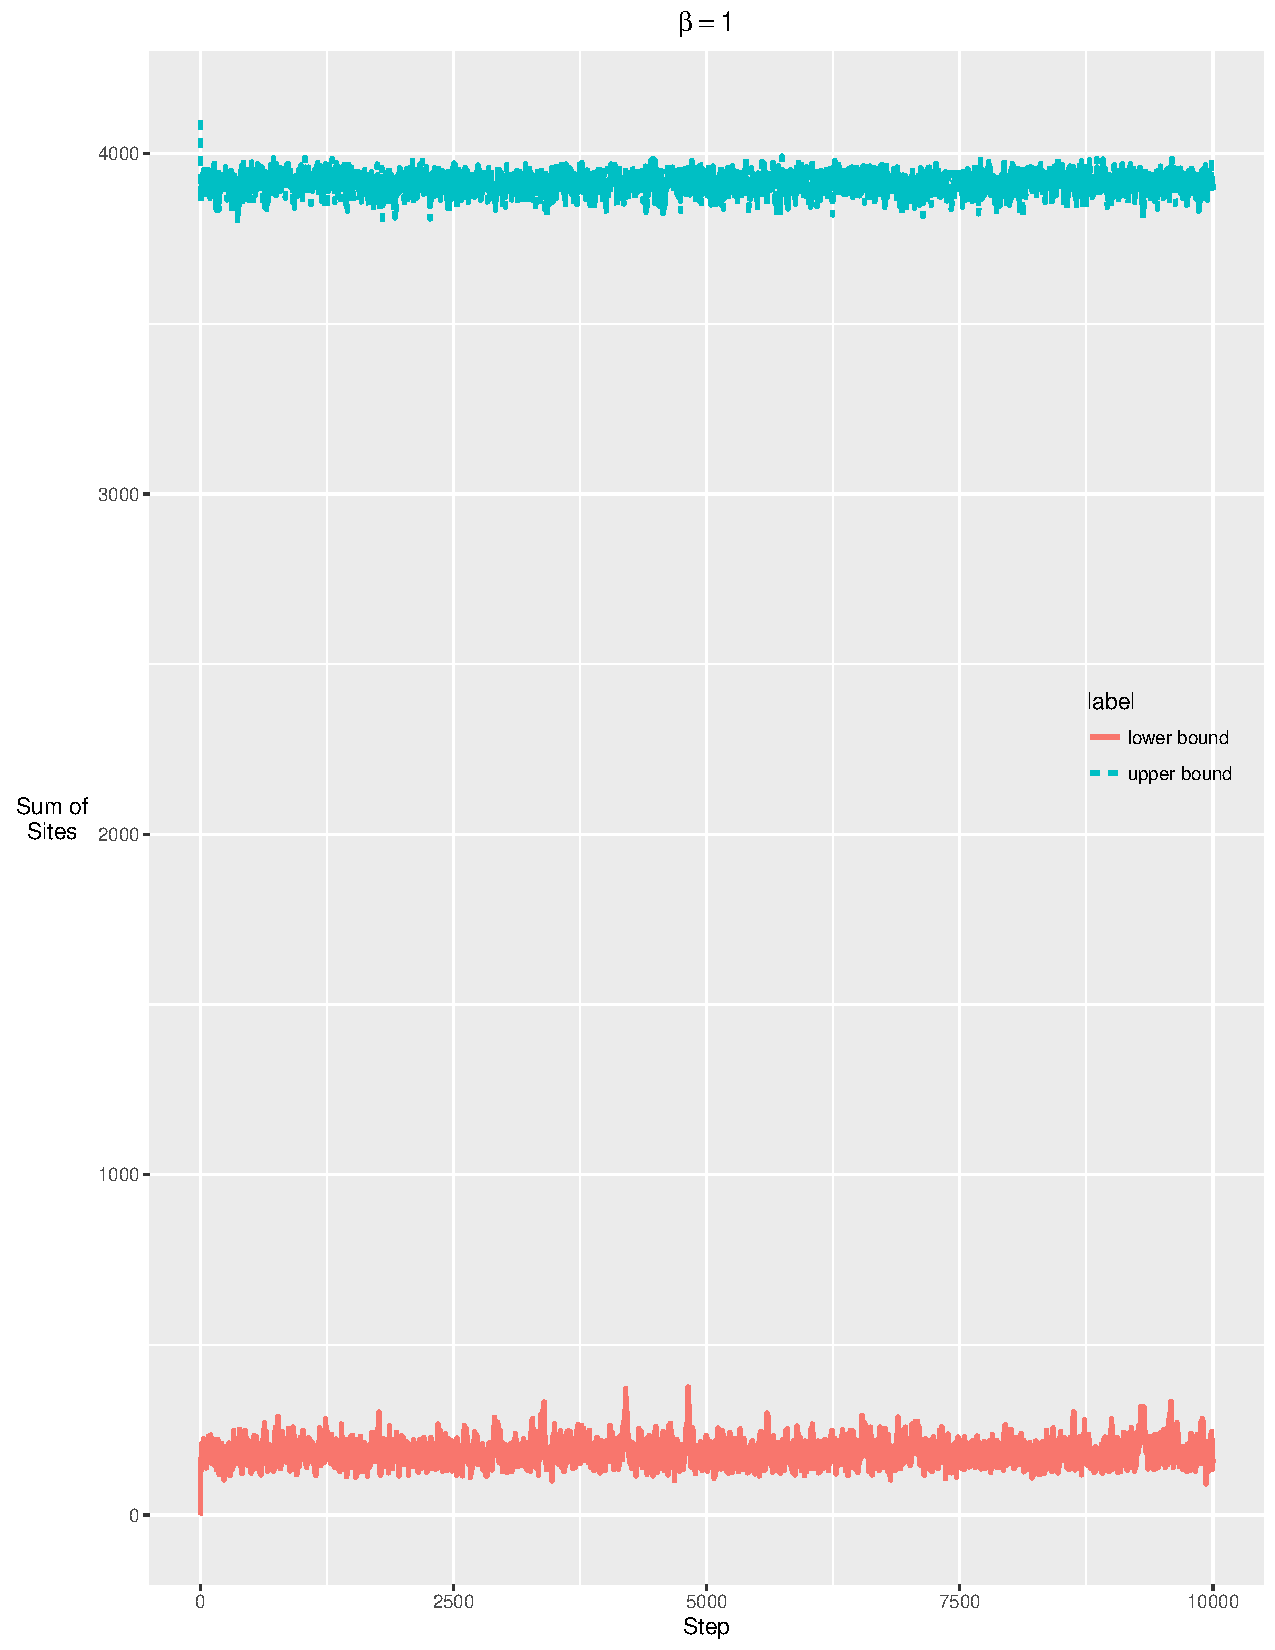
\includegraphics[width=\textwidth, height=0.5\textheight]{100.pdf}
        \end{subfigure} \\
\end{figure}

3)\par
For the second graph, we scale y-axis with log function.  So even the increasing rate of $tau$ increases exponentially with respect to $beta$.   
\begin{figure}[H]
        \centering
        \begin{subfigure}[b]{0.475\textwidth}
            \centering
            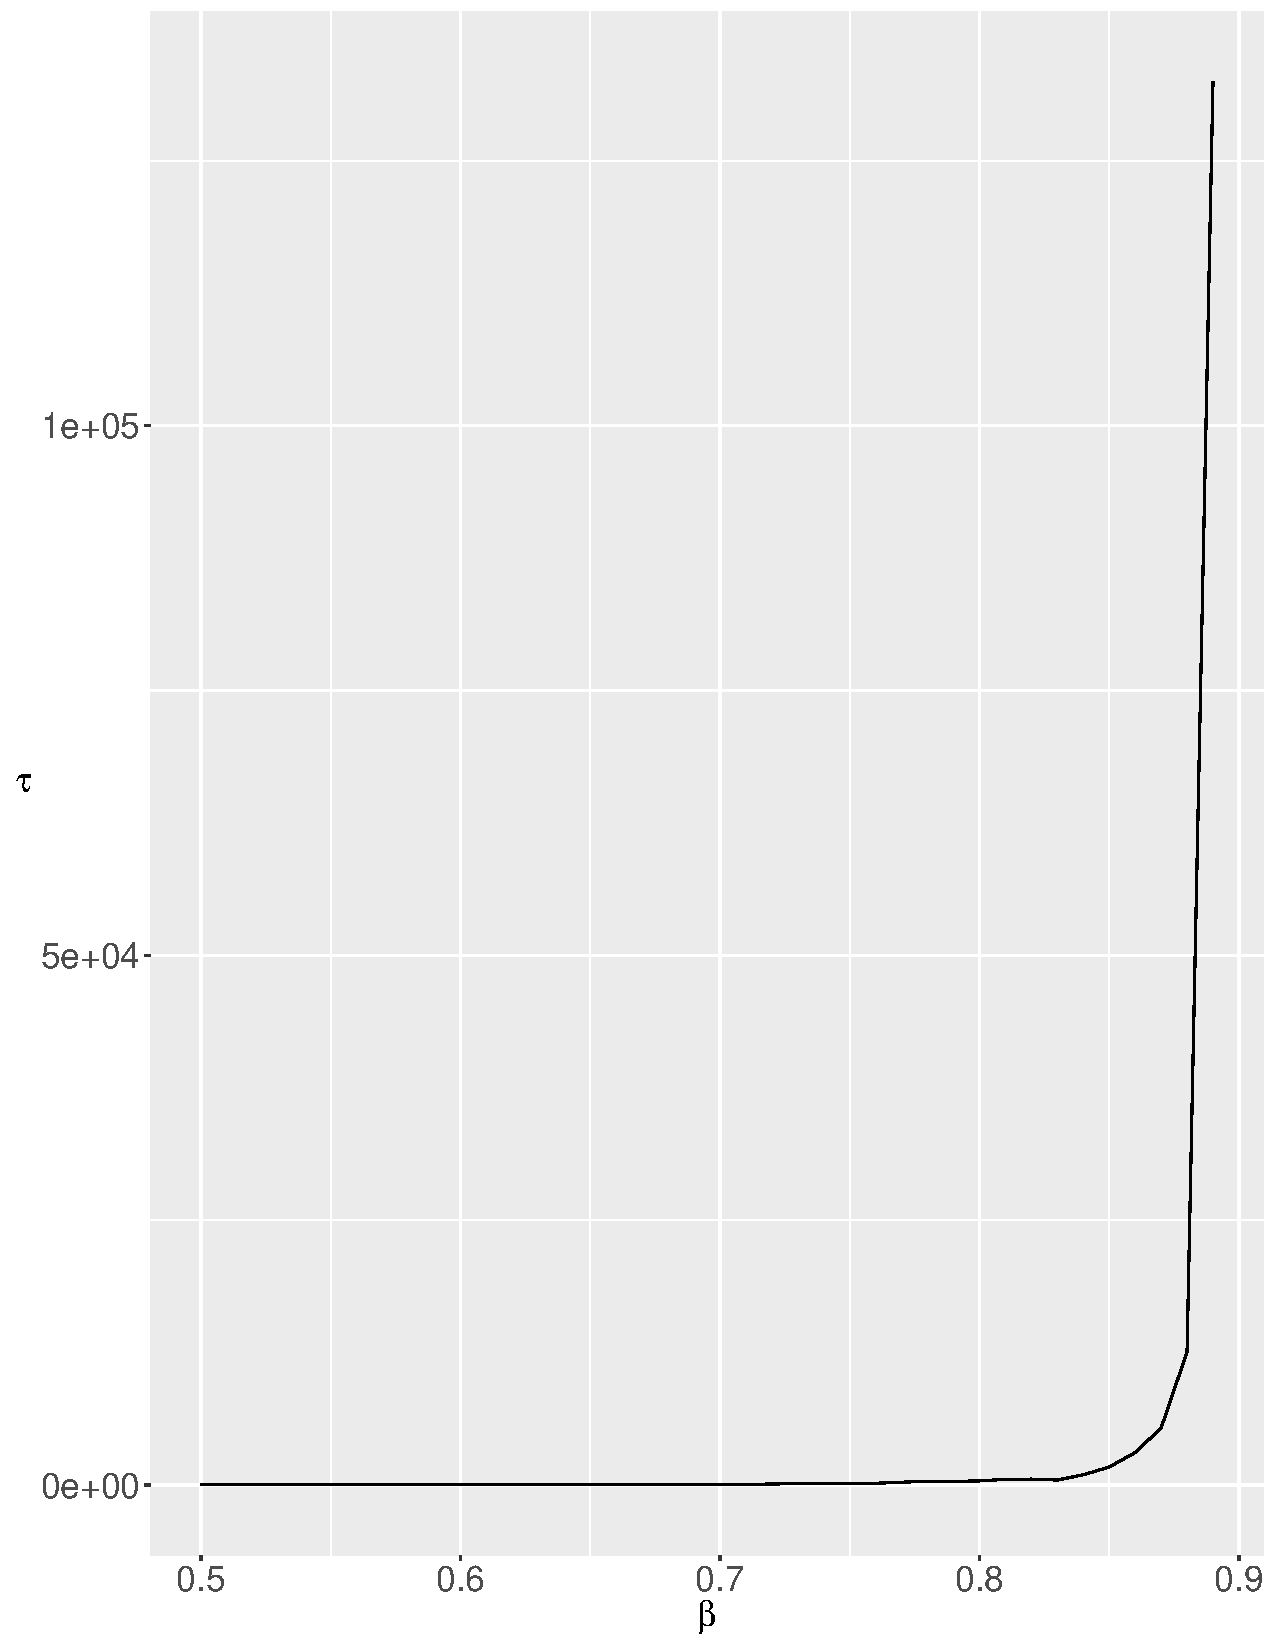
\includegraphics[width=\textwidth, height=0.5\textheight]{1.pdf}
        \end{subfigure}
        \quad
        \begin{subfigure}[b]{0.475\textwidth}
            \centering
            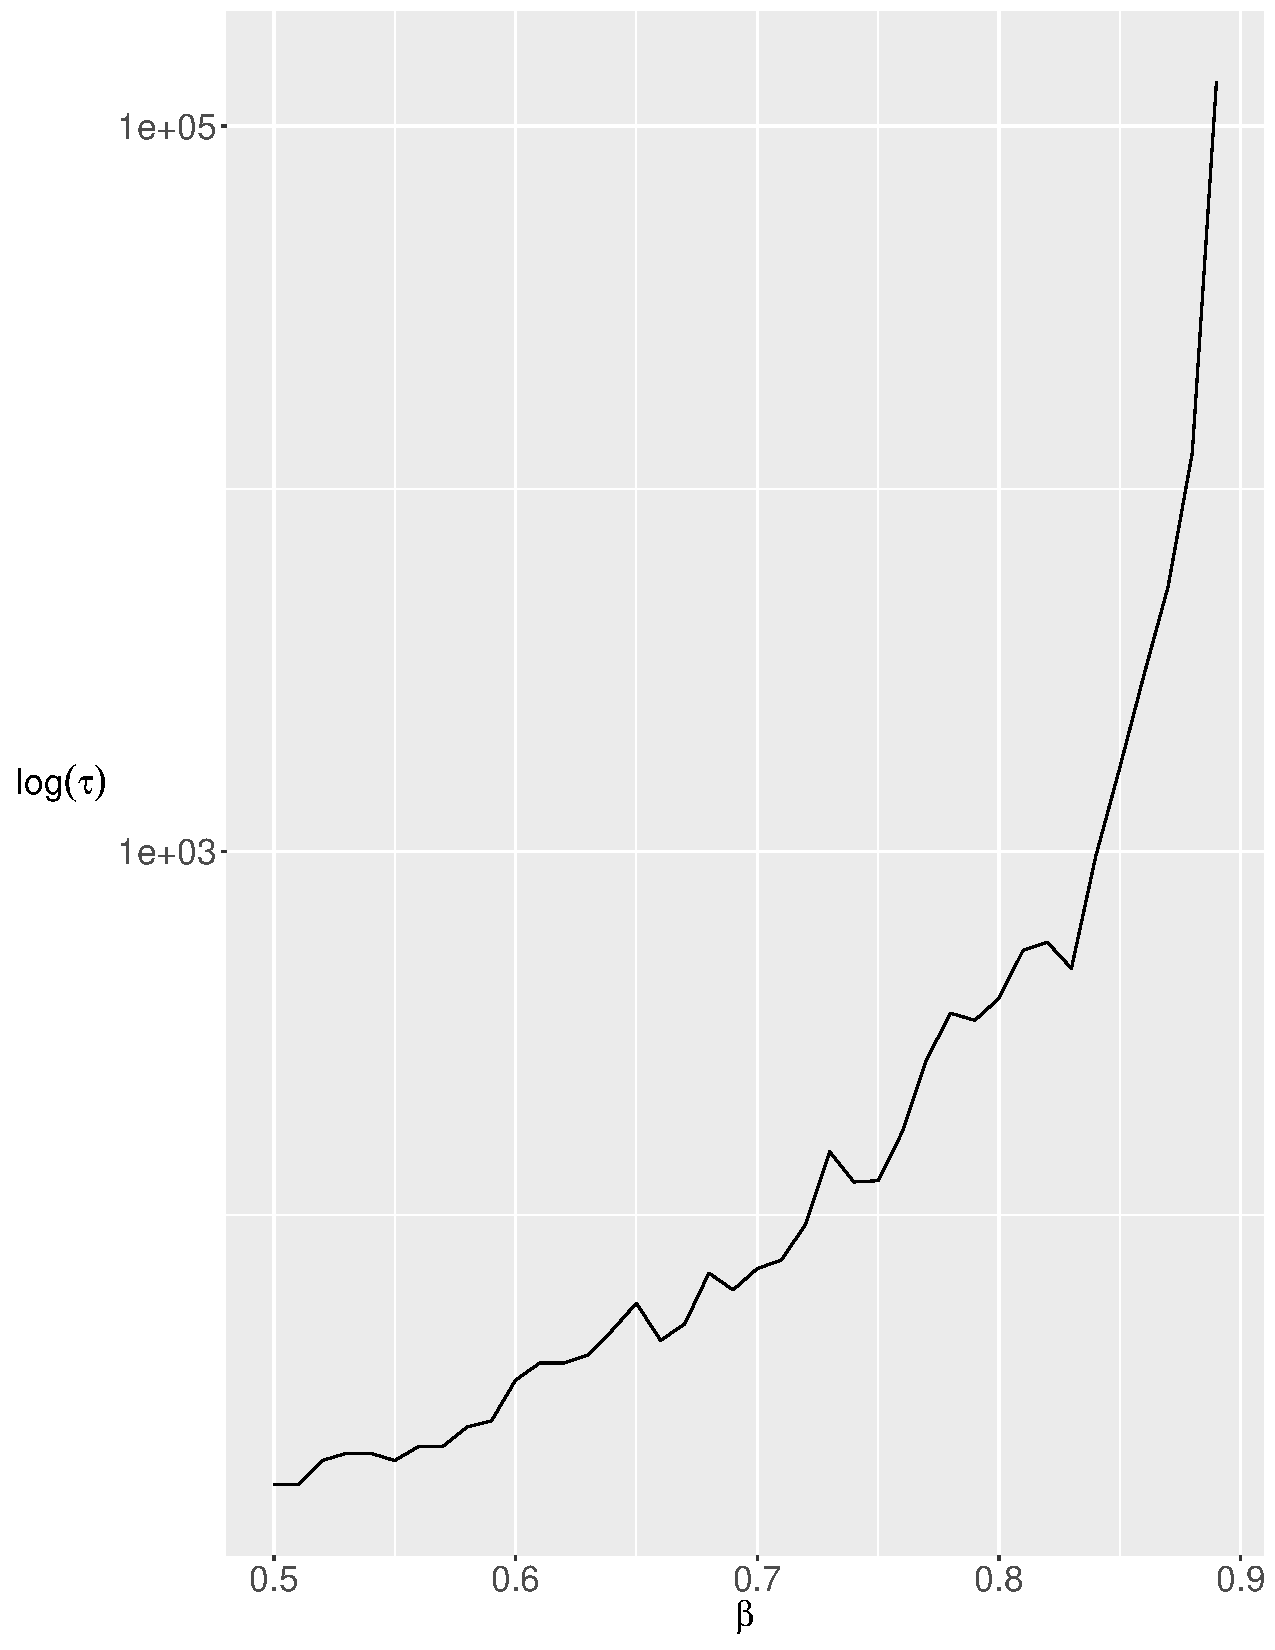
\includegraphics[width=\textwidth, height=0.5\textheight]{2.pdf}
        \end{subfigure} 
\end{figure}



\end{document}
